\documentclass[11pt, a4]{article}
\usepackage{qtree}
\usepackage{amsmath}
\usepackage{amssymb}
\usepackage{mathtools}
\usepackage{tikz}
\usepackage{forest}

\usetikzlibrary{positioning}
\newcommand\tab[1][0.5cm]{\hspace*{#1}}

%% define left/right/full outer join symbols
\def\ojoin{\setbox0=\hbox{$\bowtie$}%
  \rule[-.02ex]{.25em}{.4pt}\llap{\rule[\ht0]{.25em}{.4pt}}}
\def\leftouterjoin{\mathbin{\ojoin\mkern-5.8mu\bowtie}}
\def\rightouterjoin{\mathbin{\bowtie\mkern-5.8mu\ojoin}}
\def\fullouterjoin{\mathbin{\ojoin\mkern-5.8mu\bowtie\mkern-5.8mu\ojoin}}
\newcommand*{\QEDB}{\null\nobreak\hfill\ensuremath{\square}}%
\newcommand{\car}[1]{\tiny\textcolor{red}{#1}}
\setcounter{section}{5}
\begin{document}
\title{Exercise Sheet 6}

\section{Exercise Sheet 6}
\subsection{Exercise 1}
$|R_0| = 20, |R_1| = 10, |R_2| = 50, |R_3| = 40, |R_4| = 50, |R_5| = 55, |R_6| = 50, |R_7| = 60$\\
$f_{0,1} = 0.1, f_{0,2} = 0.2, f_{0,6} = 0.2, f_{6,7} = 0.2, f_{2,5} = 0.2, f_{2,3} = 0.2, f_{3,4} = 0.3$

\subsubsection{Give the precedence graph rooted in $R_0$}
\begin{forest}
[$R_0$
    [$R_1$,edge=-> ]
    [$R_2$,edge=-> 
        [$R_3$,edge=->
            [$R_4$,edge=-> ]
        ]
        [$R_5$,edge=-> ]
    ] 
    [$R_6$,edge=->
        [$R_7$,edge=-> ]
    ]
]
\end{forest}

\subsubsection{Perform the IKKBZ algorithm Root at $R_0$}
\begin{forest}
[$R_0$
    [$R_1$,edge=-> ]
    [$R_2$,edge=-> 
        [$R_3$,edge=->
            [$R_4$,edge=-> ]
        ]
        [$R_5$,edge=-> ]
    ] 
    [$R_6$,edge=->
        [$R_7$,edge=-> ]
    ]
]
\end{forest}
\vspace{.2cm}\\
\begin{tabular}{|c|c|c|c|c|c|}
\hline
Relation & n & s & C & T & rank\\
\hline
$R_1$ & 10 & $0.1$ & 1 & 1 & $0$\\
$R_2$ & 50 & $0.2$ & 10 & 10 & $\frac{9}{10} = 0.9$\\
$R_3$ & 40 & $0.2$ & 8 & 8 & $\frac{7}{8} = 0.875$\\
$R_4$ & 50 & $0.3$ & 15 & 15 & $\frac{14}{15} = 0.933$\\
$R_5$ & 55 & $0.2$ & 11 & 11 & $\frac{10}{11} = 0.909$\\
$R_6$ & 50 & $0.2$ & 10 & 10 & $\frac{9}{10} = 0.9$\\
$R_7$ & 60 & $0.2$ & 12 & 12 & $\frac{11}{12} = 0.917$\\
\hline
\end{tabular}
\vspace{.2cm}\\
\begin{forest}
[$R_0$
    [$R_1$,edge=-> ]
    [$R_2$,edge=-> 
        [$R_3$,edge=->
            [$R_5$,edge=->
                [$R_4$,edge=-> ]
            ]
        ]
    ] 
    [$R_6$,edge=->
        [$R_7$,edge=-> ]
    ]
]
\end{forest}
\tab $\longrightarrow$ Merge $R_2$ and $R_3$ $\longrightarrow$ \tab
\begin{forest}
[$R_0$
    [$R_1$,edge=-> ]
    [$R_{2,3}$,edge=-> 
        [$R_5$,edge=->
            [$R_4$,edge=-> ]
        ]
    ] 
    [$R_6$,edge=->
        [$R_7$,edge=-> ]
    ]
]
\end{forest}
\vspace{.2cm}\\
\begin{tabular}{|c|c|c|c|c|c|}
\hline
Relation & n & s & C & T & rank\\
\hline
$R_1$ & 10 & $0.1$ & 1 & 1 & $0$\\
$R_4$ & 50 & $0.3$ & 15 & 15 & $\frac{14}{15} = 0.933 $\\
$R_5$ & 55 & $0.2$ & 11 & 11 & $\frac{10}{11} = 0.909 $\\
$R_6$ & 50 & $0.2$ & 10 & 10 & $\frac{9}{10} = 0.9 $\\
$R_7$ & 60 & $0.2$ & 12 & 12 & $\frac{11}{12} = 0.917 $\\
$R_{2,3}$ &  &  & 90 & 80 & $\frac{79}{90} = 0.878 $\\
\hline
$R_2$ & 50 & $0.2$ & 10 & 10 & $\frac{9}{10} = 0.9 $\\
$R_3$ & 40 & $0.2$ & 8 & 8 & $\frac{7}{8} = 0.875 $\\
\hline
\end{tabular}
\vspace{.2cm}\\
\begin{forest}
[$R_0$
    [$R_1$,edge=->
        [$R_{2,3}$,edge=-> 
            [$R_6$,edge=->
                [$R_5$,edge=->
                    [$R_7$,edge=-> 
                        [$R_4$,edge=-> ]
                    ]
                ]
            ] 
        ]
    ]
]
\end{forest}
\tab $\longrightarrow$ denormalizing $\longrightarrow$ \tab
\begin{forest}
[$R_0$
    [$R_1$,edge=->
        [$R_2$,edge=-> 
            [$R_3$,edge=-> 
                [$R_6$,edge=->
                    [$R_5$,edge=->
                        [$R_7$,edge=-> 
                            [$R_4$,edge=-> ]
                        ]
                    ]
                ] 
            ]
        ]
    ]
]
\end{forest}
\vspace{1cm}\\
Resulting Join Tree =\\
\tab$((((((R_0 \bowtie R_1) \bowtie R_2) \bowtie R_3) \bowtie R_6) \bowtie R_5) \bowtie R_7) \bowtie R_4 = RJT$
\vspace{1cm}\\
$M = R_0 \bowtie R_1 $\\
$C_{out}(M) = |R_0| * |R_1| * s_1 = 20 $\\
\\
%%20
$P = (R_0 \bowtie R_1) \bowtie R_2 $\\
$C_{out}(P) = |M| * |R_2| * s_2 + C_{out}(M) = 220 $\\
%%200
\\
$Q = ((R_0 \bowtie R_1) \bowtie R_2) \bowtie R_3 $\\
$C_{out}(Q) = |P| * |R_3| * s_3 + C_{out}(P) = 1'820 $\\
%%1'600
\\
$S = (((R_0 \bowtie R_1) \bowtie R_2) \bowtie R_3) \bowtie R_6 $\\
$C_{out}(S) = |Q| * |R_6| * s_6 + C_{out}(Q) = 17'820 $\\
%%16'000
\\
$T = ((((R_0 \bowtie R_1) \bowtie R_2) \bowtie R_3) \bowtie R_6) \bowtie R_5 $\\
$C_{out}(T) = |S| * |R_5| * s_5 + C_{out}(S) = 193'820 $\\
%%176'000
\\
$U = (((((R_0 \bowtie R_1) \bowtie R_2) \bowtie R_3) \bowtie R_6) \bowtie R_5) \bowtie R_7 $\\
$C_{out}(U) = |T| * |R_7| * s_7 + C_{out}(T) = 2'305'820 $\\
%%2'112'000
\\
$C_{out}(RJT) = |U| * |R_4| * s_4 + C_{out}(U) \mathbf{= 33'985'820} $
%%31'680'000

\subsubsection{Perform the MVP algorithm}
There are no edges with weights $< 1$, so we start with phase 2:\\
Weighted-Join-Graph $G$:\\
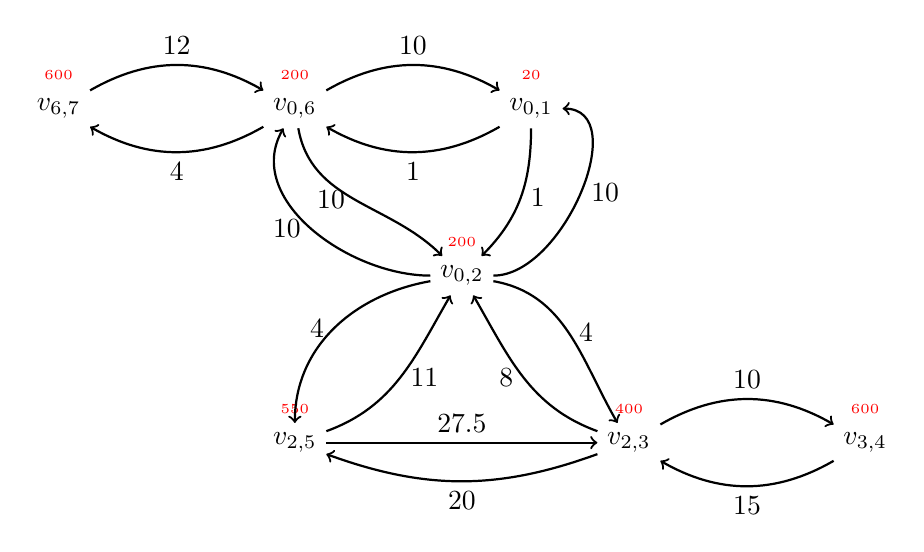
\begin{tikzpicture}[node distance=3cm]
  \node (v67) at (0,0) {$v_{6,7}$};
  \node (v67car) [above = 0cm of v67] {\car{600}};

  \node (v06) [right of=v67] {$v_{0,6}$};
  \node (v06car) [above = 0cm of v06] {\car{200}};

  \node (v01) [right of=v06] {$v_{0,1}$};
  \node (v01car) [above = 0cm of v01] {\car{20}};

  \node (v02) [below right of=v06] {$v_{0,2}$};
  \node (v02car) [above = 0cm of v02] {\car{200}};

  \node (v25) [below left of=v02] {$v_{2,5}$};
  \node (v25car) [above = 0cm of v25] {\car{550}};

  \node (v23) [below right of=v02] {$v_{2,3}$};
  \node (v23car) [above = 0cm of v23] {\car{400}};

  \node (v34) [right of=v23] {$v_{3,4}$};
  \node (v34car) [above = 0cm of v34] {\car{600}};

  \draw [->,thick] (v67) to [out=30,in=150] node[above] {12} (v06);
  \draw [->,thick] (v06) to [out=210,in=330] node[below] {4} (v67);

  \draw [->,thick] (v06) to [out=30,in=150] node[above] {10} (v01);
  \draw [->,thick] (v01) to [out=210,in=330] node[below] {1} (v06);

  \draw [->,thick] (v01) to [out=270,in=45] node[right] {1} (v02);
  \draw [->,thick] (v02) to [out=360,in=0] node[right] {10} (v01);

  \draw [->,thick] (v06) to [out=280,in=135] node[left] {10} (v02);
  \draw [->,thick] (v02) to [out=180,in=240] node[left] {10} (v06);

  \draw [->,thick] (v02) to [out=190,in=90] node[left] {4} (v25);
  \draw [->,thick] (v25) to [out=20,in=240] node[right] {11} (v02);

  \draw [->,thick] (v25) to [out=0,in=180] node[above] {27.5} (v23);
  \draw [->,thick] (v23) to [out=200,in=340] node[below] {20} (v25);

  \draw [->,thick] (v02) to [out=350,in=120] node[right] {4} (v23);
  \draw [->,thick] (v23) to [out=160,in=300] node[left] {8} (v02);
  
  \draw [->,thick] (v23) to [out=30,in=150] node[above] {10} (v34);
  \draw [->,thick] (v34) to [out=210,in=330] node[below] {15} (v23);
\end{tikzpicture}\\
Spanning Tree $S$:\\
\begin{tikzpicture}[node distance=3cm]
  \node (v67) at (0,0) {$v_{6,7}$};
  \node (v06) [right of=v67] {$v_{0,6}$};
  \node (v01) [right of=v06] {$v_{0,1}$};
  \node (v02) [below right of=v06] {$v_{0,2}$};
  \node (v25) [below left of=v02] {$v_{2,5}$};
  \node (v23) [below right of=v02] {$v_{2,3}$};
  \node (v34) [right of=v23] {$v_{3,4}$};
\end{tikzpicture}\\
%% ###########
%% STEP 1
%% ###########
\rule{\textwidth}{0.4pt}
$Q_1 = \emptyset$\\
$Q_2 = \{v_{0,1}, v_{0,6}, v_{0,2}, v_{2,3}, v_{2,5}, v_{3,4}, v_{6,7}\}$\\
Consider edge $v_{0,1} \rightarrow v_{0,2}$.\\
New cost: $\text{cost}(v_{0,1}') = 10 \cdot \frac{1}{10} \cdot 20 \cdot \frac{1}{5} \cdot 50 + 20 + 200 = 420$\\
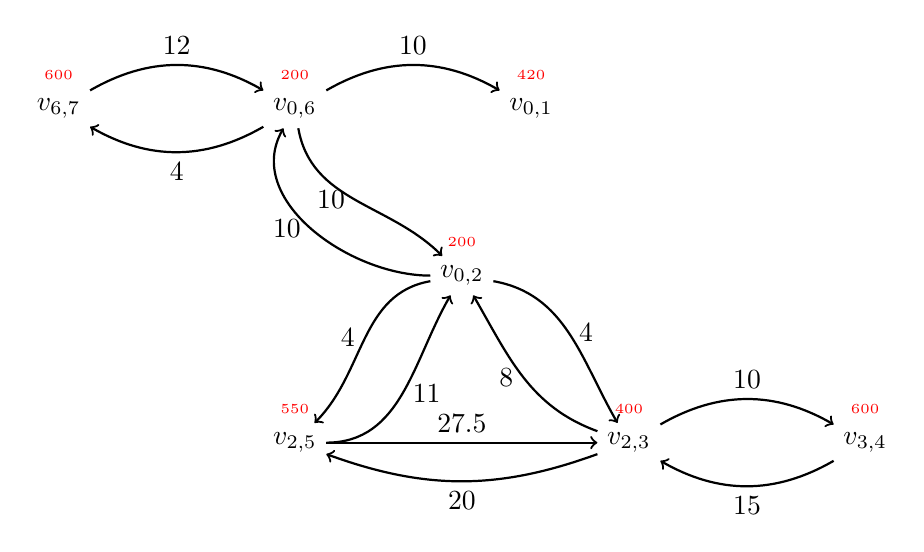
\begin{tikzpicture}[node distance=3cm]
  \node (v67) at (0,0) {$v_{6,7}$};
  \node (v67car) [above = 0cm of v67] {\car{600}};

  \node (v06) [right of=v67] {$v_{0,6}$};
  \node (v06car) [above = 0cm of v06] {\car{200}};

  \node (v01) [right of=v06] {$v_{0,1}$};
  \node (v01car) [above = 0cm of v01] {\car{420}};

  \node (v02) [below right of=v06] {$v_{0,2}$};
  \node (v02car) [above = 0cm of v02] {\car{200}};

  \node (v25) [below left of=v02] {$v_{2,5}$};
  \node (v25car) [above = 0cm of v25] {\car{550}};

  \node (v23) [below right of=v02] {$v_{2,3}$};
  \node (v23car) [above = 0cm of v23] {\car{400}};

  \node (v34) [right of=v23] {$v_{3,4}$};
  \node (v34car) [above = 0cm of v34] {\car{600}};

  \draw [->,thick] (v67) to [out=30,in=150] node[above] {12} (v06);
  \draw [->,thick] (v06) to [out=210,in=330] node[below] {4} (v67);

  \draw [->,thick] (v06) to [out=30,in=150] node[above] {10} (v01);


  \draw [->,thick] (v06) to [out=280,in=135] node[left] {10} (v02);
  \draw [->,thick] (v02) to [out=180,in=240] node[left] {10} (v06);

  \draw [->,thick] (v02) to [out=190,in=45] node[left] {4} (v25);
  \draw [->,thick] (v25) to [out=360,in=240] node[right] {11} (v02);

  \draw [->,thick] (v25) to [out=0,in=180] node[above] {27.5} (v23);  
  \draw [->,thick] (v23) to [out=200,in=340] node[below] {20} (v25);    

  \draw [->,thick] (v02) to [out=350,in=120] node[right] {4} (v23);
  \draw [->,thick] (v23) to [out=160,in=300] node[left] {8} (v02);
  
  \draw [->,thick] (v23) to [out=30,in=150] node[above] {10} (v34);
  \draw [->,thick] (v34) to [out=210,in=330] node[below] {15} (v23);

\end{tikzpicture}\\
Spanning Tree $S$:\\
\begin{tikzpicture}[node distance=3cm]
  \node (v67) at (0,0) {$v_{6,7}$};
  \node (v06) [right of=v67] {$v_{0,6}$};
  \node (v01) [right of=v06] {$v_{0,1}$};
  \node (v02) [below right of=v06] {$v_{0,2}$};
  \node (v25) [below left of=v02] {$v_{2,5}$};
  \node (v23) [below right of=v02] {$v_{2,3}$};
  \node (v34) [right of=v23] {$v_{3,4}$};

  \draw [->,thick] (v01) to [out=270,in=45] (v02);
\end{tikzpicture}\\
%% ###########
%% STEP 2
%% ###########
\rule{\textwidth}{0.4pt}
$Q_1 = \emptyset$\\
$Q_2 = \{v_{0,6}, v_{0,2}, v_{2,3}, v_{2,5}, v_{3,4}, v_{6,7}\}$\\
Consider edge $v_{0,6} \rightarrow v_{6,7}$.\\
New cost: $\text{cost}(v_{0,6}') = 60 \cdot \frac{1}{5} \cdot 50 \cdot \frac{1}{5} \cdot 20 + 600 + 200 = 3200$\\
\begin{tikzpicture}[node distance=3cm]
  \node (v67) at (0,0) {$v_{6,7}$};
  \node (v67car) [above = 0cm of v67] {\car{600}};

  \node (v06) [right of=v67] {$v_{0,6}$};
  \node (v06car) [above = 0cm of v06] {\car{3200}};

  \node (v01) [right of=v06] {$v_{0,1}$};
  \node (v01car) [above = 0cm of v01] {\car{420}};

  \node (v02) [below right of=v06] {$v_{0,2}$};
  \node (v02car) [above = 0cm of v02] {\car{200}};

  \node (v25) [below left of=v02] {$v_{2,5}$};
  \node (v25car) [above = 0cm of v25] {\car{550}};

  \draw [->,thick] (v25) to [out=0,in=180] node[above] {27.5} (v23);
  \draw [->,thick] (v23) to [out=200,in=340] node[below] {20} (v25);

  \node (v23) [below right of=v02] {$v_{2,3}$};
  \node (v23car) [above = 0cm of v23] {\car{400}};

  \node (v34) [right of=v23] {$v_{3,4}$};
  \node (v34car) [above = 0cm of v34] {\car{600}};

  \draw [->,thick] (v02) to [out=180,in=240] node[left] {10} (v06);

  \draw [->,thick] (v02) to [out=190,in=45] node[left] {4} (v25);
  \draw [->,thick] (v25) to [out=360,in=240] node[right] {11} (v02);

  \draw [->,thick] (v02) to [out=350,in=120] node[right] {4} (v23);
  \draw [->,thick] (v23) to [out=160,in=300] node[left] {8} (v02);
  
  \draw [->,thick] (v23) to [out=30,in=150] node[above] {10} (v34);
  \draw [->,thick] (v34) to [out=210,in=330] node[below] {15} (v23);

  \draw [dashed, ->,thick] (v67) to [out=280,in=190] node[left] {1} (v02);
  \draw [dashed, ->,thick] (v67) to [out=30,in=150] node[above] {1} (v01);

\end{tikzpicture}\\
Spanning Tree $S$:\\
\begin{tikzpicture}[node distance=3cm]
  \node (v67) at (0,0) {$v_{6,7}$};
  \node (v06) [right of=v67] {$v_{0,6}$};
  \node (v01) [right of=v06] {$v_{0,1}$};
  \node (v02) [below right of=v06] {$v_{0,2}$};
  \node (v25) [below left of=v02] {$v_{2,5}$};
  \node (v23) [below right of=v02] {$v_{2,3}$};
  \node (v34) [right of=v23] {$v_{3,4}$};

  \draw [->,thick] (v01) to [out=270,in=45] (v02);
  \draw [->,thick] (v06) to  (v67);
\end{tikzpicture}\\
%% ###########
%% STEP 3
%% ###########
\rule{\textwidth}{0.4pt}
$Q_1 = \emptyset$\\
$Q_2 = \{v_{0,2}, v_{2,3}, v_{2,5}, v_{3,4}, v_{6,7}\}$\\
Consider edge $v_{0,2} \rightarrow v_{2,5}$.\\
New cost: $\text{cost}(v_{0,2}') = 20 \cdot \frac{1}{5} \cdot 50 \cdot \frac{1}{5} \cdot 55 + 200 + 550= 2950 $\\
\begin{tikzpicture}[node distance=3cm]
  \node (v67) at (0,0) {$v_{6,7}$};
  \node (v67car) [above = 0cm of v67] {\car{600}};

  \node (v06) [right of=v67] {$v_{0,6}$};
  \node (v06car) [above = 0cm of v06] {\car{3200}};

  \node (v01) [right of=v06] {$v_{0,1}$};
  \node (v01car) [above = 0cm of v01] {\car{420}};

  \node (v02) [below right of=v06] {$v_{0,2}$};
  \node (v02car) [above = 0cm of v02] {\car{2950}};

  \node (v25) [below left of=v02] {$v_{2,5}$};
  \node (v25car) [above = 0cm of v25] {\car{550}};

  \draw [->,thick] (v25) to [out=0,in=180] node[above] {27.5} (v23);
  \draw [->,thick] (v23) to [out=200,in=340] node[below] {20} (v25);

  \node (v23) [below right of=v02] {$v_{2,3}$};
  \node (v23car) [above = 0cm of v23] {\car{400}};

  \node (v34) [right of=v23] {$v_{3,4}$};
  \node (v34car) [above = 0cm of v34] {\car{600}};

  
  \draw [->,thick] (v23) to [out=160,in=300] node[left] {8} (v02);
  
  \draw [->,thick] (v23) to [out=30,in=150] node[above] {10} (v34);
  \draw [->,thick] (v34) to [out=210,in=330] node[below] {15} (v23);

  \draw [dashed, ->,thick] (v67) to [out=280,in=190] node[left] {1} (v02);
  \draw [dashed, ->,thick] (v67) to [out=30,in=150] node[above] {1} (v01);

  \draw [dashed, ->,thick] (v25) to [out=90,in=270] node[right] {1} (v06);

\end{tikzpicture}\\
Spanning Tree $S$:\\
\begin{tikzpicture}[node distance=3cm]
  \node (v67) at (0,0) {$v_{6,7}$};
  \node (v06) [right of=v67] {$v_{0,6}$};
  \node (v01) [right of=v06] {$v_{0,1}$};
  \node (v02) [below right of=v06] {$v_{0,2}$};
  \node (v25) [below left of=v02] {$v_{2,5}$};
  \node (v23) [below right of=v02] {$v_{2,3}$};
  \node (v34) [right of=v23] {$v_{3,4}$};

  \draw [->,thick] (v01) to (v02);
  \draw [->,thick] (v06) to (v67);
  \draw [->,thick] (v02) to (v25);
\end{tikzpicture}\\
%% ###########
%% STEP 4
%% ###########
\rule{\textwidth}{0.4pt}
$Q_1 = \emptyset$\\
$Q_2 = \{v_{2,3}, v_{2,5}, v_{3,4}, v_{6,7}\}$\\
Consider edge $v_{2,3} \rightarrow v_{0,2}$.\\
New cost: $\text{cost}(v_{2,3}') = 20 \cdot \frac{1}{5} \cdot 50 \cdot \frac{1}{5} \cdot 40 + 2950 + 400 = 4950 $\\
\begin{tikzpicture}[node distance=3cm]
  \node (v67) at (0,0) {$v_{6,7}$};
  \node (v67car) [above = 0cm of v67] {\car{600}};

  \node (v06) [right of=v67] {$v_{0,6}$};
  \node (v06car) [above = 0cm of v06] {\car{3200}};

  \node (v01) [right of=v06] {$v_{0,1}$};
  \node (v01car) [above = 0cm of v01] {\car{420}};

  \node (v02) [below right of=v06] {$v_{0,2}$};
  \node (v02car) [above = 0cm of v02] {\car{2950}};

  \node (v25) [below left of=v02] {$v_{2,5}$};
  \node (v25car) [above = 0cm of v25] {\car{550}};

  \draw [->,thick] (v25) to [out=0,in=180] node[above] {27.5} (v23);

  \node (v23) [below right of=v02] {$v_{2,3}$};
  \node (v23car) [above = 0cm of v23] {\car{4950}};

  \node (v34) [right of=v23] {$v_{3,4}$};
  \node (v34car) [above = 0cm of v34] {\car{600}};


  \draw [->,thick] (v34) to [out=210,in=330] node[below] {15} (v23);


  \draw [dashed, ->,thick] (v67) to [out=30,in=150] node[above] {1} (v01);

  \draw [dashed, ->,thick] (v25) to [out=90,in=270] node[right] {1} (v06);

  \draw [dashed, ->,thick] (v02) to [out=350,in=90] node[above] {1} (v34);


\end{tikzpicture}\\
Spanning Tree $S$:\\
\begin{tikzpicture}[node distance=3cm]
  \node (v67) at (0,0) {$v_{6,7}$};
  \node (v06) [right of=v67] {$v_{0,6}$};
  \node (v01) [right of=v06] {$v_{0,1}$};
  \node (v02) [below right of=v06] {$v_{0,2}$};
  \node (v25) [below left of=v02] {$v_{2,5}$};
  \node (v23) [below right of=v02] {$v_{2,3}$};
  \node (v34) [right of=v23] {$v_{3,4}$};

  \draw [->,thick] (v01) to (v02);
  \draw [->,thick] (v06) to (v67);
  \draw [->,thick] (v02) to (v25);
  \draw [->,thick] (v23) to (v02);
\end{tikzpicture}\\
%% ###########
%% STEP 5
%% ###########
\rule{\textwidth}{0.4pt}
$Q_1 = \emptyset$\\
$Q_2 = \{v_{2,5}, v_{3,4}, v_{6,7}\}$\\
Consider edge $v_{2,5} \rightarrow v_{0,6}$.\\
New cost: $\text{cost}(v_{2,5}') = 50 \cdot \frac{1}{5} \cdot 55 \cdot 20 \cdot \frac{1}{5} \cdot 50 + 550 + 3200 = 113750$\\
\begin{tikzpicture}[node distance=3cm]
  \node (v67) at (0,0) {$v_{6,7}$};
  \node (v67car) [above = 0cm of v67] {\car{600}};

  \node (v06) [right of=v67] {$v_{0,6}$};
  \node (v06car) [above = 0cm of v06] {\car{3200}};

  \node (v01) [right of=v06] {$v_{0,1}$};
  \node (v01car) [above = 0cm of v01] {\car{420}};

  \node (v02) [below right of=v06] {$v_{0,2}$};
  \node (v02car) [above = 0cm of v02] {\car{2950}};

  \node (v25) [below left of=v02] {$v_{2,5}$};
  \node (v25car) [above = 0cm of v25] {\car{113750}};



  \node (v23) [below right of=v02] {$v_{2,3}$};
  \node (v23car) [above = 0cm of v23] {\car{4950}};

  \node (v34) [right of=v23] {$v_{3,4}$};
  \node (v34car) [above = 0cm of v34] {\car{600}};

  \draw [->,thick] (v34) to [out=210,in=330] node[below] {15} (v23);
  \draw [dashed, ->,thick] (v67) to [out=30,in=150] node[above] {1} (v01);
  \draw [dashed, ->,thick] (v02) to [out=350,in=90] node[above] {1} (v34);

\end{tikzpicture}\\
Spanning Tree $S$:\\
\begin{tikzpicture}[node distance=3cm]
  \node (v67) at (0,0) {$v_{6,7}$};
  \node (v06) [right of=v67] {$v_{0,6}$};
  \node (v01) [right of=v06] {$v_{0,1}$};
  \node (v02) [below right of=v06] {$v_{0,2}$};
  \node (v25) [below left of=v02] {$v_{2,5}$};
  \node (v23) [below right of=v02] {$v_{2,3}$};
  \node (v34) [right of=v23] {$v_{3,4}$};

  \draw [->,thick] (v01) to (v02);
  \draw [->,thick] (v06) to (v67);
  \draw [->,thick] (v02) to (v25);
  \draw [->,thick] (v23) to (v02);
  \draw [->,thick] (v25) to (v06);
\end{tikzpicture}\\
%% ###########
%% STEP 6
%% ###########
\rule{\textwidth}{0.4pt}
$Q_1 = \emptyset$\\
$Q_2 = \{v_{3,4}, v_{6,7}\}$\\
Consider edge $v_{3,4} \rightarrow v_{2,3}$.\\
New cost: $\text{cost}(v_{3,4}') = 50 \cdot \frac{3}{10} \cdot 40 \cdot \frac{1}{5} \cdot 50 + 600 + 4950 = 11550$\\
\begin{tikzpicture}[node distance=3cm]
  \node (v67) at (0,0) {$v_{6,7}$};
  \node (v67car) [above = 0cm of v67] {\car{600}};

  \node (v06) [right of=v67] {$v_{0,6}$};
  \node (v06car) [above = 0cm of v06] {\car{3200}};

  \node (v01) [right of=v06] {$v_{0,1}$};
  \node (v01car) [above = 0cm of v01] {\car{420}};

  \node (v02) [below right of=v06] {$v_{0,2}$};
  \node (v02car) [above = 0cm of v02] {\car{2950}};

  \node (v25) [below left of=v02] {$v_{2,5}$};
  \node (v25car) [above = 0cm of v25] {\car{113750}};

  \node (v23) [below right of=v02] {$v_{2,3}$};
  \node (v23car) [above = 0cm of v23] {\car{4950}};

  \node (v34) [right of=v23] {$v_{3,4}$};
  \node (v34car) [above = 0cm of v34] {\car{11550}};

  \draw [dashed, ->,thick] (v67) to [out=30,in=150] node[above] {1} (v01);
  \draw [dashed, ->,thick] (v02) to [out=350,in=90] node[above] {1} (v34);

\end{tikzpicture}\\
Spanning Tree $S$:\\
\begin{tikzpicture}[node distance=3cm]
  \node (v67) at (0,0) {$v_{6,7}$};
  \node (v06) [right of=v67] {$v_{0,6}$};
  \node (v01) [right of=v06] {$v_{0,1}$};
  \node (v02) [below right of=v06] {$v_{0,2}$};
  \node (v25) [below left of=v02] {$v_{2,5}$};
  \node (v23) [below right of=v02] {$v_{2,3}$};
  \node (v34) [right of=v23] {$v_{3,4}$};

  \draw [->,thick] (v01) to (v02);
  \draw [->,thick] (v06) to (v67);
  \draw [->,thick] (v02) to (v25);
  \draw [->,thick] (v23) to (v02);
  \draw [->,thick] (v25) to (v06);
  \draw [->,thick] (v34) to (v23);
\end{tikzpicture}\\
spanning tree is complete $\Rightarrow$ stop.\\
Resulting join tree:\\

%% tree
\Tree[.$\bowtie$
        [.$\bowtie$
            [.$\bowtie$ 
                [.$\bowtie$
                    [.$\bowtie$ 
                      [.$\bowtie$
                        $R_3$
                        $R_4$
                      ]
                      $R_2$
                    ]
                    [.$\bowtie$ 
                      $R_0$
                      $R_1$
                    ]
                ]
                $R_5$
            ]
            $R_6$
        ]
        $R_7$
]

\end{document}
